\section{Obliczenia MES i wyznaczanie krzywych dyspersji oraz wzbudzalności}
\label{cha:obliczenia_mes}

W tej sekcji przedstawione są kolejno sposoby tworzenia siatki węzłów, budowy elementów skończonych, wyznaczania lokalnych i globalnych macierzy modelu MES pręta i wyznaczani krzywych dyspersji oraz wzbudzalności. Program umożliwia tworzenie modelu MES z wykorzystanie elementów czworościennych oraz sześciennych. Krzywe dyspersji oraz wzbudzalności można wyznaczyć z obliczonego modelu, ale jest też opcja wczytania danych modelu z programu MARC.

Strukturę projektu przedstawia rysunek \ref{fig:okno_projektu}. Implementacja zagadnień związanych z obliczeniami MES oraz wyznaczaniem krzywych dyspersji z obliczonego modelu znajduje się w katalogu MES\textunderscore dir. Katalog MARC zawiera funkcje umożliwiające wczytanie danych z programu MARC i na ich podstawie wyznaczeniu krzywych dyspersji.

\begin{figure}[h]
\centering
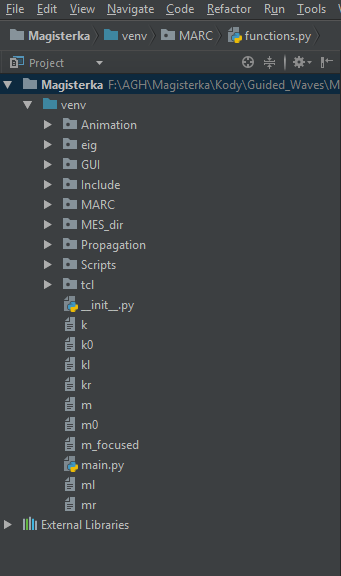
\includegraphics[width=5cm]{Zdjecia/5/okno_projektu}
\caption{Widok okna projektu}
\label{fig:okno_projektu}
\end{figure}

\subsection{Elementy czworościenne}
\label{cha:elementy czworościenne}

Zawartość katalogu MES dir przedstawia rysunek \ref{fig:okno_projektu_MES}. Obliczenia dotyczące elementów czworościennych zawarte są w modułach katalogu tetrahedralElements. Poniżej znajdują się funkcje poszcególnych modułów, wraz z opisem ich zastosowania, argumentami wejściowymi oraz wyjściowymi.

\begin{figure}[h]
\centering
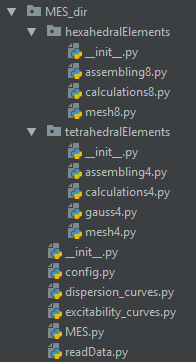
\includegraphics[width=5cm]{Zdjecia/5/okno_projektu_MES}
\caption{Widok okna projektu}
\label{fig:okno_projektu_MES}
\end{figure}


 \( \textbf{Moduł mesh4} \).

\textit{circlePlaneVerticies(x, radius, numberOfPoints)} - funkcja wykorzystywana przy tworzeniu siatki (w circleMeshFull oraz circleMeshSparse). Dodaje do siatki węzły na okręgu w płaszczyźniej pręta na długości x. Promień okręgu określa radius, a ilość węzłów na okręgu to numberOfPoints.

\textit{circleMeshFull(radius, numberOfCircles, numberOfPoints)} - funkcja tworzy siatkę na trzech płaszczyznach przesuniętych o 1 we współrzędnej x. Siatka zbudowana jest na każdej płaszczyźnie tak samo i zawiera węzeł centralny oraz okręgi z węzłami w ilości numberOfCircles. Na każdym okręgu liczba węzłów jest większa, aby zapewnić możliwie równe odległości pomiędzy węzłami. Pierwszy okrąg zawiera liczbę węzłów numberOfPoints. Zwraca tablicę o wymiarach n x 3, gdzie n to liczba węzłów. W kolumnach są kolejne współrzędne węzłów.

\textit{circleMeshSparse(radius, numberOfCircles, numberOfPoints)} - jak wyżej, z tą różnicą, że każdy okrąg siatki ma tyle samo węzłów.

\textit{triangulation(vertices)} - funkcja tworzy elementy skończone czworościenne. Przyjmuje macierz węzłów z powyższych funkcji i zwraca tablicę e x 4, gdzie e to liczba elementów. W kolumnach zawarte są indeksy węzłów z macierzy wejściowej, które należą do danego elementu.

\textit{correctVolumeSign(vertices, indices)} - funkcja sprawdza czy objętość elementu skończonego obliczona za pomocą wyznacznika ma dodatnią wartość. Jeśli nie, to zmienia miejscami dwa indeksy elementu w macierzy zwróconej z triangulation(vertices).

\textit{drawPlane(vertices)} - funkcja przyjmuje macierz węzłów i rysuje ich układ na płaszczyźnie. Przykładowe układu przedstawione są na rysunku \ref{fig:siatka}.

\textit{drawBar(vertices)} - funkcja przyjmuje macierz węzłów i rysuje wszystkie węzły w rzucie izometrycznym. Przykład przedstawia rysunek \ref{fig:pret}.

\textit{drawTriangulation(vertices, indices)} - funkcja przyjmuje macierz węzłów i macierz elementów skończonych. Rysuje elementy skończone w rzucie izometrycznym. Przykład przedstawia rysunek \ref{fig:triangulation}.

\begin{figure}
\begin{subfigure}{.5\textwidth}
  \centering
  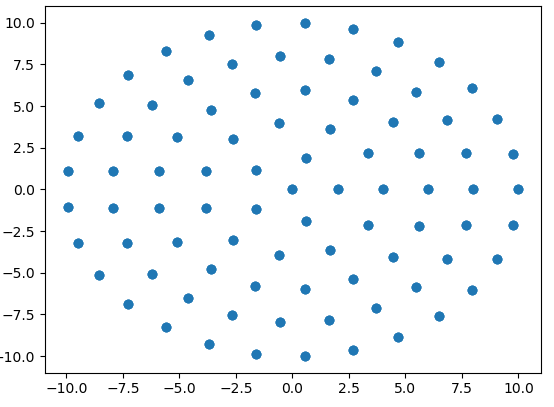
\includegraphics[width=.8\linewidth]{Zdjecia/5/siatka1}
  \caption{}
  \label{fig:sfig1}
\end{subfigure}%
\begin{subfigure}{.5\textwidth}
  \centering
  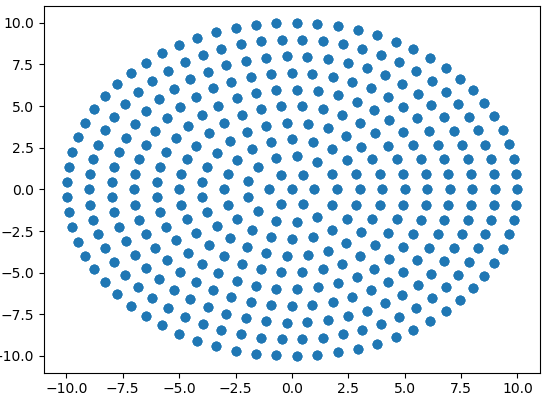
\includegraphics[width=.8\linewidth]{Zdjecia/5/siatka2}
  \caption{}
  \label{fig:sfig2}
\end{subfigure}\\
\begin{subfigure}{.5\textwidth}
  \centering
  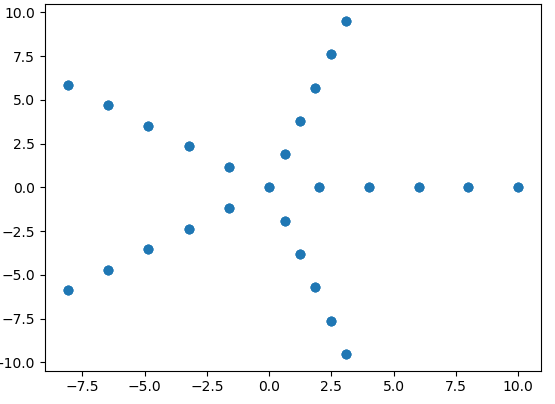
\includegraphics[width=.8\linewidth]{Zdjecia/5/siatka3}
  \caption{}
  \label{fig:sfig3}
\end{subfigure}%
\begin{subfigure}{.5\textwidth}
  \centering
  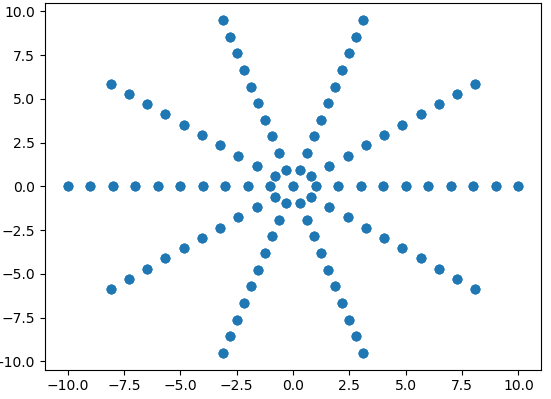
\includegraphics[width=.8\linewidth]{Zdjecia/5/siatka4}
  \caption{}
  \label{fig:sfig4}
\end{subfigure} 
\caption{Układ siatki węzłów na płaszczyźnie powstałych z a) \textit{circleMeshFull(10, 5, 5)} b) \textit{circleMeshFull(10, 10, 10)} c) \textit{circleMeshSparse(10, 10, 10)} d) \textit{circleMeshSparse(10, 10, 10)}}
\label{fig:siatka}
\end{figure}


\begin{figure}
\begin{subfigure}{.5\textwidth}
  \centering
  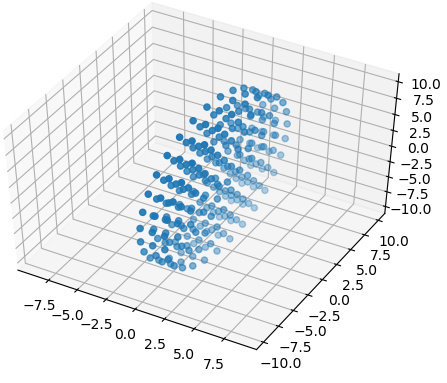
\includegraphics[width=.8\linewidth]{Zdjecia/5/pret1}
  \caption{}
  \label{fig:sfig1}
\end{subfigure}%
\begin{subfigure}{.5\textwidth}
  \centering
  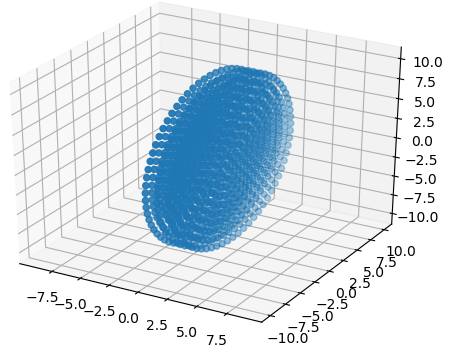
\includegraphics[width=.8\linewidth]{Zdjecia/5/pret2}
  \caption{}
  \label{fig:sfig2}
\end{subfigure}\\
\begin{subfigure}{.5\textwidth}
  \centering
  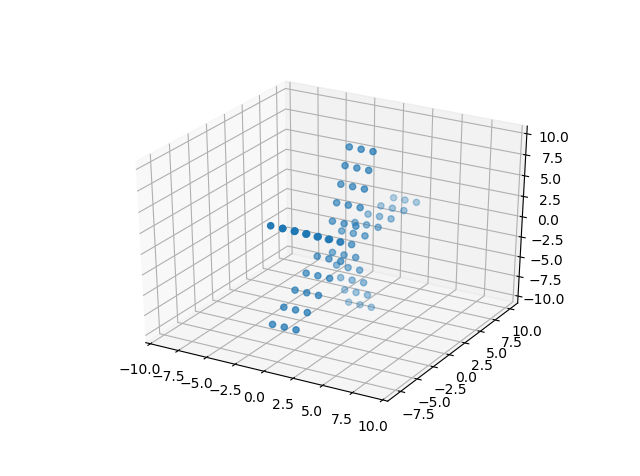
\includegraphics[width=.8\linewidth]{Zdjecia/5/pret3}
  \caption{}
  \label{fig:sfig3}
\end{subfigure}%
\begin{subfigure}{.5\textwidth}
  \centering
  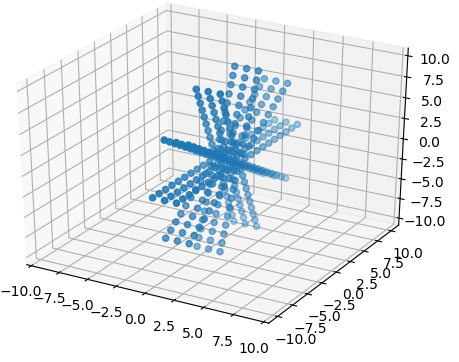
\includegraphics[width=.8\linewidth]{Zdjecia/5/pret4}
  \caption{}
  \label{fig:sfig4}
\end{subfigure} 
\caption{Układ siatki węzłów pręta z a) \textit{circleMeshFull(10, 5, 5)} b) \textit{circleMeshFull(10, 10, 10)} c) \textit{circleMeshSparse(10, 10, 10)} d) \textit{circleMeshSparse(10, 10, 10)}}
\label{fig:pret}
\end{figure}

\begin{figure}
\begin{subfigure}{.5\textwidth}
  \centering
  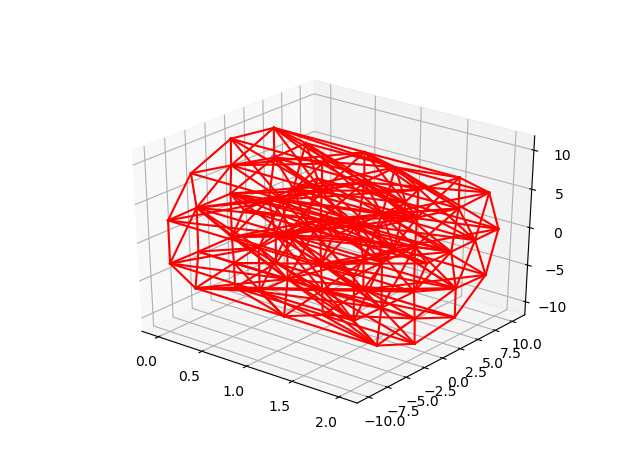
\includegraphics[width=.8\linewidth]{Zdjecia/5/triangulation1}
  \caption{}
  \label{fig:sfig1}
\end{subfigure}%
\begin{subfigure}{.5\textwidth}
  \centering
  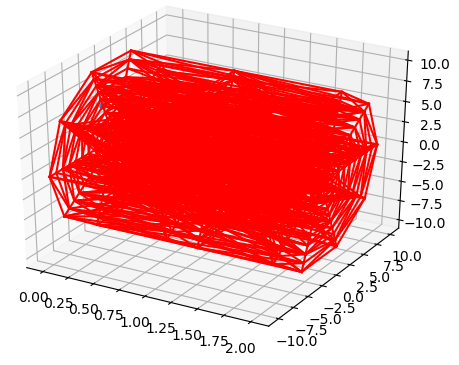
\includegraphics[width=.8\linewidth]{Zdjecia/5/triangulation2}
  \caption{}
  \label{fig:sfig2}
\end{subfigure}

\caption{Triangulacja (elementy skończone) dla siatki a) \textit{circleMeshFull(10, 3, 3)} b) \textit{circleMeshSparse(10, 10, 10)}}
\label{fig:triangulation}
\end{figure}


